% File:		vtdc_power.tex
% Author:	Adam Lewis
\documentclass[preprint]{sigplanconf}
% Packages used in this document
\usepackage{cite} 
\usepackage{graphicx}
\usepackage{url}
\usepackage{amsmath}
% correct bad hyphenation here
\hyphenation{op-tical net-works semi-conduc-tor IEEEtran}

\begin{document}
% paper title
%\titlebanner{}
%\preprintfooter{}
\title{Impact of Virtualization on Server Power Consumption}
% author names and affiliations
\authorinfo{Adam Lewis \and Chris Thompson \and  Nian-Feng Tzeng \and  D'mitri Perkins}
  {Center for Advanced Computer Studies\\
    The University of Louisiana at Lafayette\\
    Lafayette, Louisiana 70508}
   {\{awlewis,cct2361,tzeng,perkins\}@cacs.louisiana.edu }
\maketitle

\begin{abstract}
\label{abstract}
Large data centers host hundreds or even thousands of servers that require
complex and costly cooling solutions.  One approach to reducing this cost and
complexity is to take advantage of virtualization techniques to run multiple
instances of server software on single physical servers to reduce the overall
power consumption.  This paper uses experiments based upon the methodology of
statistical design of experiments to investigate some of the characteristics
of virtualization and to evaluate the power consumption of virtual servers.
\end{abstract}

\section{Introduction}
\label{sec:Introduction}
The heart of the infrastructure of today's information economy is the
data centers containing the servers that support most Internet services.
Such centers host hundreds or even thousands of servers running off-the-shelf
hardware.   The power demands of these installations force firms to install
complex and costly cooling solutions to efficiently move the heat away from
servers so as to avoid reliability problems.

Providing proper cooling has become more difficult as the density of the
off-the-shelf hardware has increased with tighter packaging, decreasing form
factors, and increasing performance demands.  The introduction of multi-core
processors combined together in clusters of traditional and blade servers has
greatly increased the power demands of servers.

Two approaches have been taken towards managing the power
consumption of microprocessors.   Once approach has been the application of
dynamic voltage scaling: reducing the voltage (and as a result, the frequency)
of the processor at he cost slower program execution.   Other approaches (such
as taken by Intel with the Pentium 4 processors) have utilized a stop-go
approach: activate and deactivate the processor as demanded by workload.

These approaches have mostly been applied to battery-powered devices.   They
adjust components to lowest power-mode that does not over-compromise
performance.    These transitions occur based on analysis of workload or
higher-level operation.

Server systems, per \cite{Bianchini2004}, have characteristics that make
traditional power management techniques undesirable:
\begin{itemize}
\item server hardware is typically provisioned for peak load, and thus
  exhibit high performance and power consumption;
\item high availability and high bandwidth is typically provided by widespread
  replication of resources such as clusters of machine and disk arrays;
\item server power supplies must be able to store capacity to deal with sudden
  spikes in load and as result exhibit high power losses.
\end{itemize}

Application servers pose an especially interesting power management problem due
to intensive CPU and memory requirements combined with maintaining soft state
that is not typically replicated.   Intensive CPU and memory use means that
traditional power management mechanisms may impose too excessive demands upon
performance while non-replicated state forces state migration in order to turn
application servers on and off.

One approach to dealing with the spiraling complexity in the data center is
virtualiztion: presenting a logical grouping or subset of computing resources
in a manner that provides benefits over the original configuration.
Virtualization software simulates the hardware in a manner that allows a
``guest'' operating system to operate as if it was running on the bare
hardware.

\section{Motivation}
\label{sec:Motivation}
Extensive research has occurred into the design and manufacture of energy and
temperature efficient microprocessors.   As multi-core
microprocessors become more prevalent, computer architects have been exploring
energy and thermal techniques required to effectively manage the energy
consumption of multi-core processors \cite{Donald2006}.

Vitrualization has a long history in the operating system community beginning
with the IBM VM/370 commercial product \cite{Gum1983}.  In recent times,
commercial systems such as VMware \cite{VMWare2005} and open source systems
such as Bochs \cite{Bochs2006} have implemented virtualization systems on the
Intel x86 architecture.

A common concept amongst these systems is the idea of a ``hypervisor'' which
is the underlying piece of software responsible for managing and scheduling
the different virtual machines running on a single processor.  The hypervisor
is responsible for managing the physical resources shared amongst the virtual
machines. 

The virtualization systems we have introduced so far provide ``full
virtualization'' of the physical hardware.  They must provide a complete
simulation of the environment.  Recently, systems such as the open source
``Xen'' environment \cite{Barham2003} \cite{Abels2005} and the commercial
Parallels Desktop \cite{parallels2006} have popularized the concept of
``paravirtualization'' where the guest operating system is provided with an
abstraction that is similar but not identical to the underlying physical
hardware.  As such, guest operating systems must be aware that are executing
on a virtual machine.  The advantage is that the guest can achieve performance
levels approaching that of executing on the physical hardware.

\begin{figure*}
  \centering
    \includegraphics[scale=0.65]{graphics/xen3arch.eps}
  \label{fig:XenArch}
  \caption{Xen 3.0 System Architecture \cite{Xen2006}}
\end{figure*}
In this work, we use the Xen virtualization system \cite{Barham2003} as the
starting point for our investigation into virtual machine performance.   Xen
was developed with the idea that it was one piece of the control systems
required to build an ``Internet-scale'' computing infrastructure.  This is
important when we consider being able to provide the application developer
with the view of a large collection of resources that are locally available.

The workloads typical of an application server in a computing cluster and grid
often are very different than the common workload mixes in a single computer
environment.   Virtualization can provide high-performance computing
environments with services beyond just consolidation as it allows
\emph{specialization} \cite{Mergen2006}.  By consolidating physical access to
the devices within the hypervisor, it allows one to tailor allocation of those
resources at a much finer grain layer than what is possible with legacy
operating systems while permitting the application developer to maintain some
compatibility with legacy, commodity operating system.

\section{Virtualization and Power Management}
\label{sec:PowerMgt}
The conceptual model provided to the application developer by virtualization
is quite seductive.  From an application standpoint, all resources appear to
be local and we leave it up the hypervisor to handle the scheduling and
allocation of resources.  Our inspiration is the XenoServer \cite{Fraser2003}
and VMPlant projects \cite{Krsul2004}.   Furthermore, providing a means for
the high-performance computing application to coexist with minimal
interference with a commodity operating system reduces the cost and complexity
of the high-performance application \cite{Mergen2006}.

So, given an hypervisor capable of scheduling virtual machines amongst either
multiple cores within the single die of a processor or a traditional symmetric
multiprocessing system, what is the power consumption of a node in this network
given the workloads expressed by a typical parallel processing benchmark in a
virtualized environment.

A virtualized configuration raises some interesting questions when considering
power management.   First, what happens when both operating system in the
hypervisor and the operating system in the virtual machine try to optimize
workloads to reduce power consumption?  Second, can we achieve a better
solution by just letting the hypervisor exclusively handle power management?

It should be noted that even though the focus of this research is upon
minimizing the power consumption and controlling the resource allocation of
computing power, similar techniques can be applied to controlling other
resources within the machine (memory or disk drives, for example).

\section{Design of Experiments}
\label{sec:DoE}
Statistical Design of Experiment (DoE) \cite{Montgomery2005} is a methodology
to efficiently determine the effects input factors have upon one or more
response metrics.  There are three principles in DoE: Replication,
Randomization, and Blocking.  Replication ensures that the results were not a
fluke and reduces the error.  Randomization ensures that no unintended bias is
introduced by uncontrollable factors.  Blocking organizes the trials so that
common factors can be examined concurrently.

There are two types of input factors, qualitative and quantitative.
Quantitative factors are those that can be given a value like number of
wireless nodes or distance from a gateway.  Qualitative factors are those
which cannot be given a value as in surface terrain or routing protocol.  The
R-Squared value tells us how much of the variability in our data can be
contributed to the input factors.

A factorial design consists several input factors are tested at different
levels to and the response metrics are examined.  Each input factor typically
has two levels, a high and a low.  Other common designs include three level
factors and mixed level factors.  Full factorial design means that all
possible combination of factors are tested.  In a $2^{3}$ experiment, 8 trials
are performed.  In a half factorial design, only 4 trials would be performed.
This is done when there is not enough time or resources available to complete
all of the trials.

Once all of the trials have been completed, Analysis of Variance is performed
to determine the factor effects and regression model.  The factor effects tell
us what main effects (those based on individual factors) and interaction
effects (those based on the interaction between the individual factors) are
important to our regression model.  The regression model will give us a
formula that can be used to estimate the response metric based on the input
factors without running any experiments.  DoE has an advantage of typical
one-factor-at-a-time experiments in that it observes the effect of the
interactions of the input factors.  These factors are often overlooked in
one---factor--at--a--time experiments and could be the most important effect
in the regression model.

A set of experiments has been performed to investigate the impact of
virtualization on power management.  We test the hypothesis that it is
more efficient to concentrate power management functionality within the
hypervisor than allowing both the hypervisor and virtual machines to attempt
to manage power consumption. 

\section{Experimental Results}
\label{sec:Results}
Our first experiment investigated whether or not the power consumed by the
processor varied if a single benchmark was executed on a physical processor or
on the same processor running on a single virtual machine.As a follow-up test, we investigated the impact of varying the mix of integer and floating point
instructions on the power consumption if we include the Xen
hypervisor modules in the Linux kernel.  

We attempt to answer this question by
executing a \(2^{2}\) full factorial experiment.  The results of this
experiment prompted further investigation with a \(3^{2}\) mixed-level
factorial experiment that examined the instruction mix in more detail. The
third experiment was a \(2^{3}\) experiment that examined how different
combinations of instruction mix and use of virtual machines impacted the power
consumed by the test hardware.

\subsection{Experiment Setup and Data Collection}
\label{sec:Setup}
Our experiments take physical measurements of the power consumed by executing
a collection of benchmark programs selected from the SPEC CPU2000
benchmark suite.   The benchmarks were
chosen due to prior work \cite{Donald2006} finding those benchmarks drove
the targeted processors to a steady state temperature.

The benchmark programs were assigned to run as independent processes either on
the domain0 physical machine (i.e., the hypervisor) or on a domainU (virtual
machine) controlled by the domain0 machine.   The programs are executed by a
driver script that runs on the domain0 machine and are started on the domainU
machines using an SSH connection.   We assume that the power consumption due
to the overhead of this script and running the programs via SSH is minimal.

The power consumed is measured with a WattsUP \cite{WattsUp2006a} power meter
that is connected between the AC Main and our test hardware.  The power meter
measures the total and average wattage, voltage, and amperage over the run of
a workload.  The internal memory of the power meter is cleared at the start of
the run and the measures during the run are downloaded after the run completes
from the meter's internal memory into a relational database
\cite{WattsUp2006b}.

\begin{table*}
  \centering
  \label{tab:hardware}
  \begin{tabular}{l|l}
    \hline
    \multicolumn{2}{c}{\bf{Dell PowerEdge 6450}}\\  
    CPU&4x700MHz Pentium III Xenon\\
    CPU L2 cache&2MB\\
    Memory&4GB\\
    Internal\\disk&4x18GB\\
    Network\\ Interface Card&2x100Mbps\\
    RAID\\ controller&2xPERC 2/DC\\
    Video&On-board \\
    Height&4 rack units or 7''\\
  \end{tabular}
  \caption{Hardware configuration}
\end{table*}
Our test hardware is a Dell Poweredge 6450 configured as shown in Table 1.
The operating system used is the Fedora Core 5 distribution of Linux with
version 2174 of the Linux 2.6.17 kernel either with or without Xen kernel
enhancements depending upon the experiment.  Four identical virtual machines
were created on the server.

In each experiment, we measure \emph{power consumed} which we define as total
wattage consumed over the length of run of the workload.

\subsection{Is there an impact on power consumption using Xen}
\label{sec:XenImpact}
Our first experiment considers the overall impact on power consumption of the
hypervisor.   In this experiment, we posit the existence of a linear
relationship between the power consumed by process running in the domain0
kernel and the domainU kernel and then confirm or deny the existence of the
relationship via statistical analysis.  The experiment is shown in Table
\ref{tab:SingleTab}.

\subsubsection{Experiment Design}
The factors considered in this experiment are
\begin{list}{}{}
\item $benchmark$: A benchmark from the SPEC2000 benchmark suite selected
  based on prior work \cite{Dondald2006} that showed that executed the
  benchmark resulted in a steady state temperature in the CPU. As such, the
  benchmark also will result in consistent power consumption over multiple runs.
\item $withxen$: A binary variable indicating whether the benchmark was
  executed in the domain0 or in a single instance of a domainU virtual machine.
\end{list}
The quantity measured in the experiment was the total wattage consumed during
the run of the program.   The proposed model has the form
\begin{equation*}
  \label{InitialModel1}
  Totalwatts = A*Benchmark + B*withxen
\end{equation*}
Each benchmark was executed three times within domain0 kernel and three times
with the domainU hypervisor.

\subsubsection{Estimation of parameters and analysis of variance}
The data shown in Table \ref{tab:SingleTab} was analyzed using the R statistical
software \cite{R2007}.  The fit of this data against the proposed linear
regression model is shown in Table \ref{tab:SingelModelFit}.  The companion
analysis of variance can be found in Table \ref{tab:SingleModelAnova}.  

The analysis of the data would indicate that the initial term of the model
dominates.  This implies that the benchmarks that measure the computational
performance do not consume additional power if they are executed in a virtual
machine versus the physical machine.

\subsection{Is there a relationship between Xen and instruction mix?}
\label{sec:XenAndInstructionMix}
Our second experiment considers the relationship between power consumed,
instruction mix, and whether or not the Linux kernel includes the Xen kernel
modules. We address this question with the experiment shown in Table
\ref{tab:ExperimentDesign1}.  This is a $2^{k}$ full factorial design with
$k=2$ factors with each factor assigned $2$ values or factor levels.  One
combination of factors defines a design point.  Each design point is
replicated three times.

\subsubsection{Experiment Design}

The factors considered in this experiment were 
\begin{list}{}{}
\item $IFP$: The instruction Mix measures the ratio of integer instructions in the
  workload to the number of floating point instructions.  The instruction mix
  was normalized to range between $-1<=IFP<=1$ .
\item $WXEN$: With or without Xen indicates whether the workload was executed
  with an operating system kernel that contained the Xen extensions.
\end{list}
Note that the processes that composed the workload were all executed in the
domain0 if the Xen-extended kernel was used.

\subsubsection{Estimation of Effects and Allocation of Variance}
The design matrix in Table \ref{tab:ExperimentDesign1} was analyzed using the
SAS statistical software \cite{SAS2006}.  An analysis of variance (Table
\ref{tab:AnovaExperiment1}) was performed to identify the statistically
significant effects and their interactions.  These were combined together to
build the following model:

\begin{equation*}
  \label{eq:ModelEquation1}
  TOTWATTS = 3298.167 - 112.667*IFP
\end{equation*}

The effect estimates associated with this model can be found in Table 
\ref{tab:EffectEstimates1} and a statistical analysis of the fit of the model
is in Table \ref{tab:FitStatsExperiment1}.   The statistics indicate we may
have an issue with how well our model will predict the impact on the total
wattage consumed given changes in the two inputs.  

\begin{figure*}
  \centering
  \begin{center}
    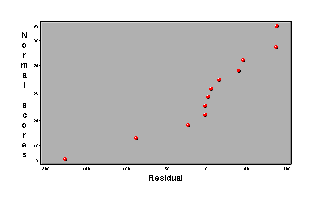
\includegraphics[scale=1.5]{graphics/normalresiduals1.eps}
  \end{center}
  \caption{Normal Probability Plot for Experiment 1}
  \label{fig:Residuals1}
\end{figure*}
Further evidence of the lack of fit can be seen in the normal probability plot of
the residuals in Figure \ref{fig:Residuals1}.  There is an assumption in DoE
\cite{Montgomery2005} that the residuals (i.e., the difference between
predicted value and the observed values) are normally distributed.  If the
residuals are plotted on the X-axis and the rank-ordered expected normal
values are plotted on the Y-axis produces a graph where the values form a
straight line, then one can be satisfied that the residuals are normally
distributed.  For this experiment, the values do not meet this criteria.

\subsection{How can we confirm our conclusions about instruction mix and Xen?}
\label{sec:XenAndInstructionMixFollowUp}
\label{Experiment2}
The data from our previous experiment indicates that including Xen support in
the kernel has statistically negligible affect upon power consumption when
considering instruction mix.  The instruction mix variable $IFP$ is a
continuous variable but we became curious about the possibility that effect on
total watts consumed was not linear in nature. Additional runs were performed
to expand our original experiment from a $2^{2}$ full factorial experiment to
a $3^{2}$ full factorial experiment.   The design of the expanded experiment
is in Table \ref{tab:ExperimentDesign2}.


\subsubsection{Estimation of Effects and Allocation of Variance}
\label{sec:Experiment2Analysis}
The design matrix in Table \ref{ExperimentDesign2} was analyzed using the
SAS statistical software \cite{SAS2006}.   A second analysis of variance was
performed to identify the statistically significant effects and their
interactions.   These were combined together to build the following model:
\begin{equation*}
  \label{eq:ModelExperiment2}
  TOTWATTS = 3273.444 - 112.667*IFP
\end{equation*}

\begin{figure*}
  \centering
  \begin{center}
    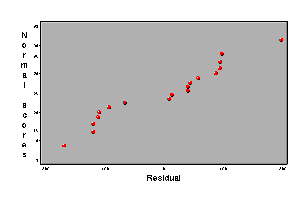
\includegraphics[scale=1.5]{graphics/normalresiduals2.eps}
  \end{center}
  \caption{Normal Probability Plot for Experiment 2}
  \label{fig:Residuals2}
\end{figure*}
A statistical analysis of the fit of the model is in Table
\ref{tab:FitStatsExperiment2}.  Note that both the $R-square$ and $Adjusted
R-square$ values for the model are worse than what we saw in our first
experiment.  The normal probability plot of the residuals for this model is
shown in Figure \ref{fig:Residuals2}.  In this case, we see a similar spread
of the residuals to the previous experiment.  Given this result, we see enough
statistical evidence to indicate that including the Xen extensions has
negligible effect on power consumption when the instruction mix is varied.

\subsection{How does different ways of using Xen affect power consumption?}
\label{sec:XenUse}
\label{Experiment3}
We address this question with the experiment shown in Table
\ref{tab:ExperimentDesign3}.  This is a $2^{k}$ full factorial design with
$k=3$ factors with each factor assigned $2$ values or factor levels.  One
combination of factors defines a design point.  Each design point is
replicated three times.

The factors considered in this experiment were 
\begin{list}{}{}
\item $IFP$: \emph{Instruction Mix} measures the ratio of integer instructions in the
  workload to the number of floating point instructions.  The instruction mix
  was normalized to range between $-1<=IFP<=1$.
\item $USEHYP$: \emph{Use of hypervisor} indicates whether or not one of the
  processes in the workload was executed in domain0.
\item $ALLIN1$: \emph{All processes executed in one VM or spread across multiple VMs}.
\end{list}

\subsubsection{Estimation of Effect and Allocation of Variance}
The SAS statistical software \cite{SAS2006} was used to analyze the experimental
results.  The main and interaction effects were analyzed using analysis of
variance (Table \ref{tab:AnovaExperiment3}) to identify those effects and
interactions that are statistically significant.  The resulting model includes
those effects and interactions that are significant to a 95\% confidence
interval:
\begin{flalign*}
  \label{eq:ModelExperiment3}
  TOTWATTS &= 3003.417 - 96.333*IFP \\
  & + 81.333*USEHYP + 108.167*ALLIN1
\end{flalign*}

\begin{figure*}
  \centering
  \begin{center}
    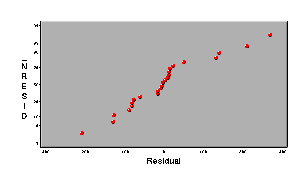
\includegraphics[scale=1.5]{graphics/normalresiduals3.eps}
  \end{center}
  \caption{Normal Probability Plot of Residuals for Experiment 3}
  \label{fig:Residuals3}
\end{figure*}
The statistical analysis of the fit of this predictive model to the data is in
Table \ref{tab:FitStatsExperiment3}.   In this case, the analysis of the fit
indicates that model is a more reasonable predictor of the impact of the input
factors on total wattage consumed.   This conclusion is supported by the
normal probability plot of the residuals in Figure \ref{fig:Residuals3}.

Recall that the instruction mix variable $IFP$ is a continuous factor
varying between $-1$ and $1$ depending upon the ratio of integer instructions
to floating point instructions.  As such, we can use our predictive model to
build the response surface shown in Figure \ref{fig:RSM3}.

\begin{figure*}
  \centering
  \begin{center}
    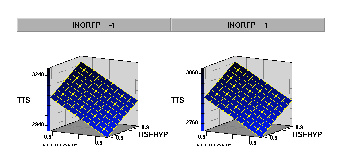
\includegraphics[scale=2.0]{graphics/surfaceplot.eps}
  \end{center}
  \caption{Response Surface for the Predictive Model in Experiment 3}
  \label{fig:RSM3}
\end{figure*}

\section{Conclusions and Future Work}
\label{sec:Conclusions}

We can draw the following conclusions from our experiments:
\begin{itemize}
\item Benchmarks that measure the computational performance of the processor
  (such as those in the SPEC2000 benchmark suite) do not appear to consume
  additional power when run in a virtual machine versus the physical hardware.
\item The power consumed depending upon varying instruction mixes is not
  affected by having the Xen hypervisor extensions included in the system kernel.
\item There is sufficient data to conclude that running processes on both the
  hypervisor and in the virtual machines impacts the power consumed.
\item Spreading the workload across all virtual machines reduces the overall
  power consumed and sufficient data exists to indicate this is independent of
  the instruction mix.
\end{itemize}

Work has begun to investigate the impact of an energy-aware hypervisor in
an single processor environment \cite{Reinhardt2005}.  The addition of an
energy-aware hypervisor capable of scheduling across multiple cores in a
single processor and across multiple processors is projected to reduce the
overall power consumption. Xen can be configured so that an individual virtual
machine can be locked onto one CPU.  Additional experiments are needed to
evaluate the power profile of this configuration.

Follow-on research is needed to consider the impact of having both domain0 and
domainU kernels attempting to manage the power consumption.  Virtualization of
 these devices adds an extra level of complexity to the hypervisor that can
be avoided if support for these functions can be left out of the domainU
kernels.

The experimental results presented in this paper provide a baseline and
testbed for evaluating the impact of other factors on power consumption of
server clusters.  In particular, the testbed presented in this paper will be
used to evaluate the impact on power consumption of enhancements to a
hyper visor's memory management scheme and virtual machine scheduling.

% references section
\label{sec:References}
\nocite{*}
\bibliographystyle{plain}
\bibliography{vtdc_power}

%Tables have now been moved to the end of the document and converted to full
%span tables.
\begin{table*}
  \centering
  \begin{tabular}{l|l|l|lll}
    benchmark&withvm&totalwatts&&\\
    \hline
    crafty&0&2851&2860&2856\\
    crafty&1&2865&2854&2861\\
    eon&0&2835&2851&2850\\
    eon&1&2837&2840&2838\\
    gcc&0&2970&2980&2979\\
    gcc&1&2986&2981&2964\\
    gzip&0&2894&2902&2892\\
    gzip&1&2893&2886&2898\\
    mcf&0&3322&3336&3333\\
    mcf&1&3338&3333&3328\\
    perlbmk&0&2906&2903&2907\\
    perlbmk&1&2898&2910&2899\\
    twolf&0&2967&2956&2947\\
    twolf&1&2947&2958&2955\\
  \end{tabular}
  \caption{Power Consumed By Selected SPEC2000 Benchmarks}
  \label{tab:SingleTab}
\end{table*}

\begin{table*}
  \centering
  \begin{tabular}{l|l|l|l|l}
     Factor&Estimate&Std. Error&t value&Pr(>|t|)    \\
     \hline
     (Intercept)&2855.667&3.786&754.358 &< 2e-16\\
     eon&-10.333&5.354&-1.930& 0.0634 \\
     gcc&121.083&5.008&24.179& < 2e-16\\
     gzip&40.333&5.354&7.534&2.64e-08 \\
     mcf&474.667&5.354& 88.663 & < 2e-16\\ 
     perlbmk&49.667&5.354&   9.277& 3.52e-10 \\
     twolf&101.000& 5.354&  18.866&  < 2e-16 \\
     withvm&4.333& 5.354&  0.809&   0.4249 \\
     eon:withvm&-11.333&7.571&  -1.497&   0.1452    \\
     gcc:withvm&-4.083&7.331&  -0.557&   0.5818    \\
     gzip:withvm&-8.000&7.571&  -1.057&   0.2994   \\
     mcf:withvm&-1.667&7.571&  -0.220&   0.8273    \\
     perlbmk:withvm&-7.333&7.571&  -0.969&   0.3408  \\  
     twolf:withvm&-7.667&7.571&  -1.013&   0.3196    \\
     \hline
     R-Squared&0.9988&&&\\
     Adj R-Squared&0.9982&&&\\
   \end{tabular}
   \caption{Effect Estimates for Linear Regression Model}
   \label{tab:SingleModelFit}
 \end{table*}

 \begin{table*}
   \centering
   \begin{tabular}{l|l|l|l|l|l}
     Factor&           Df&  Sum Sq& Mean Sq&   F value& Pr(>F)    \\
     \hline
     benchmark&         6& 1020676&  170113& 3956.9004& <2e-16\\
     withvm&           1&      20&      20&    0.4610& 0.5026  \\  
     benchmark:withvm& 6&     143&      24&    0.5542& 0.7627  \\
     Residuals&        29&    1247&      43&          &         \\
  \end{tabular}
  \caption{Analysis of Variance of the Linear Regression Model}
  \label{tab:SingleModelAnova}
\end{table*}
\clearpage
\begin{table*}
  \centering
  \begin{tabular}{l|l|l|l}
    $RUN$&$IFP$&$WXEN$&$TOTWATTS$ \\
    \hline
    2&1&-1&3066\\
    6&1&-1&3193\\
    10&1&-1&3198\\
    4&1&1&3225\\
    8&1&1&3235\\
    12&1&1&3196\\
    1&-1&-1&3450\\
    5&-1&-1&3454\\
    9&-1&-1&3450\\
    3&-1&1&3458\\
    7&-1&1&3196\\
    11&-1&1&3457\\
  \end{tabular}
  \caption{\(2^{2}\) Design Matrix and Experimental Output for Experiment 1}
  \label{tab:ExperimentDesign1}
\end{table*}

\begin{table*}
  \centering
  \begin{tabular}{llllll|lllll}
    \multicolumn{1}{c}{} & \multicolumn{5}{c|}{Master Model}&\multicolumn{5}{c}{Predictive Model} \\
    Source&$DF$&$MS$&$MS$&$F$&$PR>F$&$DF$&$SS$&$MS$&$F$&$Pr>F$ \\
    \hline
    $IFP$&1&152325.3&152325.3 &21.15164&0.001758&1&152325.3&152325.3&20.5694&0.001082 \\
    $WXEN$&1&161.3333&161.3333&0.022402&0.884726&&&&& \\
    $IFP*WXEN$&1&16280.33&16280.33&2.26066&0.171106&&&&& \\
    &&&&&&&&&& \\
    $Model$&3&168767&56255.67&7.811569&0.00921&1&152325.3&152325.3&20.5694&0.001082 \\
    $Error$&57612.67&7201.583& & &10&74054.33&7405.433&&& \\
    $Total$&11&226379.7& & & &11&226379.7&&& \\
  \end{tabular}
  \caption{ANOVA Analysis for Experiment 1}
  \label{tab:AnovaExperiment1}
\end{table*}

\begin{table*}
  \centering
  \begin{tabular}{l|llll|llll}
    \multicolumn{1}{c}{}& \multicolumn{4}{c|}{Master Model } & \multicolumn{4}{c}{Predictive Model}\\
    \hline
    \bf{Term}&\bf{Estimate}&\bf{Std Err}&\bf{t}&\bf{$Pr>|t|$}&\bf{Estimate}&\bf{Std Err}&\bf{t}&\bf{$PR>|t|$}\\
    $IFP$&-225.333&48.9958&-4.599&0.00176&-225.330&49.685&-4.535&0.001082\\
    $WXEN$&-7.333&48.995&-0.1500&0.88473&&&&\\
    $IFP*WXEN$&73.6667&48.99518&1.504&0.17110&&&\\
  \end{tabular}
  \caption{Effect Estimates for Experiment 1}
  \label{tab:EffectEstimates1}
\end{table*}


\begin{table*}
  \centering
  \label{tab:FitStatsExperiment1}
  \begin{tabular}{l|ll}
    &Master Model&Predictive Model \\
    $RMSE$&84.8621&86.0548 \\
    $R-square$&74.55\%&67.25\% \\
    $Adjusted R-square$&65.01\%&64.02\% \\
    $Coefficient of variation$&2.573&2.609 \\
  \end{tabular}
  \caption{Fit Statistics for Experiment 1}
\end{table*}
\clearpage
\begin{table*}
  \centering
  \begin{tabular}{l|ll|l}
    $RUN$&$IFP$&$WXEN$&$TOTWATTS$ \\
    \hline
    3&1&-1&3066\\
    9&1&-1&3193\\
    15&1&-1&3198\\
    6&1&1&3225\\
    12&1&1&3235\\
    18&1&1&3196\\
    28&0&-1&3494\\
    8&0&-1&3187\\
    14&0&-1&3179\\
    5&0&1&3142\\
    11&0&1&3158\\
    17&0&1&3184\\
    1&-1&-1&3450\\
    7&-1&-1&3454\\
    13&-1&-1&3450\\
    4&-1&1&3458\\
    10&-1&1&3196\\
    16&-1&1&3457\\
  \end{tabular}
  \caption{\(3^{2}\) Design Matrix and Experimental Output for Experiment 2}
  \label{tab:ExperimentDesign2}
\end{table*}


\begin{table*}
  \centering
  \begin{tabular}{llllll|lllll}
    \multicolumn{1}{c}{} & \multicolumn{5}{c|}{Master Model}&\multicolumn{5}{c}{Predictive Model} \\
    Source&$DF$&$MS$&$MS$&$F$&$PR>F$&$DF$&$SS$&$MS$&$F$&$Pr>F$ \\
    \hline
    $IFP$&1&152325.300&152325.300 &13.0392&0.00257&1&152325.300&152325.300&13.172&0.002255 \\
    $WXEN$&1&9800.000&9800&0.839&0.374&&&&& \\
    &&&&&&&&&& \\
    $Model$&2&162125.300&81062.670&6.939065&0.00735&1&152325.300&152325.300&13.1719&0.00226\\
    $Error$&15&175231.100&11682.070&&&16&185031.100&11567.440&&\\
    $(Lack of Fit)$&3&52207.110&17402.370&1.975&0.220&1&22002.780&22002.780&2.0244&0.1753\\
    $Total$&17&337356.400& & & &17&337356.400&&& \\
  \end{tabular}
  \caption{ANOVA Analysis for Experiment 2}
  \label{tab:AnovaExperiment2}
\end{table*}

\begin{table*}
  \centering
  \begin{tabular}{l|ll}
    &Master Model&Predictive Model \\
    $RMSE$&108.084&107.538\\
    $R-square$&48.06\%&45.15\% \\
    $Adjusted R-square$&41.13\%&41.72\% \\
    $Coefficient of variation$&3.301832&3.285167 \\
  \end{tabular}
  \caption{Fit Statistics for Experiment 2}
  \label{tab:FitStatsExperiment2}
\end{table*}

\begin{table*}
  \centering
  \begin{tabular}{l|llll|llll}
    \multicolumn{1}{c|}{}&\multicolumn{4}{c|}{Master Model}&\multicolumn{4}{c}{Predictive Model}\\
    \bf{Term}&\bf{Estimate}&\bf{Std Err}&\bf{t}&\bf{$Pr>|t|$}&\bf{Estimate}&\bf{Std Err}&\bf{t}&\bf{$Pr>|t|$}\\
    \hline
    $IFP$&-192.667&50.7267&-3.798&0.00144&-192.667&50.691&-3.8008&0.00112\\
    $WXEN$&-23.333&25.475&-0.916&0.374&&&&\\
  \end{tabular}
  \caption{Effect Estimate for Experiment 2}
  \label{tab:EffectEstimates2}
\end{table*}
\clearpage
\begin{table*}
  \centering
  \begin{tabular}{l|l|l|l|l}
    $RUN$&$IFP$&$USEHYP$&$ALLIN1$&$TOTWATTS$ \\
    \hline
    8&1&1&1&3071\\
    16&1&1&1&3051\\
    24&1&1&1&3032\\
    4&1&1&-1&2862\\
    12&1&1&-1&2890\\
    20&1&1&-1&3082\\
    6&1&-1&1&2929\\
    14&1&-1&1&2835\\
    22&1&-1&1&2965\\
    2&1&-1&-1&2732\\
    10&1&-1&-1&2704\\
    18&1&-1&-1& 2732\\
    7&-1&1&1&3287\\
    15&-1&1&1&3286\\
    23&-1&1&1&3282\\
    3&-1&1&-1&3063\\
    11&-1&1&-1&2847\\
    19&-1&1&-1&3264\\
    5&-1&-1&1&3464\\
    13&-1&-1&1&3069\\
    21&-1&-1&1&3068\\
    1&-1&-1&-1&2781\\
    9&-1&-1&-1&2785\\
    17&-1&-1&-1&3001\\
  \end{tabular}
  \caption{\(2^{3}\) Design Matrix and Experimental Output for Experiment 3}
  \label{tab:ExperimentDesign3}
\end{table*}

\begin{table*}
  \centering
  \begin{tabular}{llllll|lllll}
    \multicolumn{1}{c}{} & \multicolumn{5}{c|}{Master Model}&\multicolumn{5}{c}{Predictive Model} \\
    Source&$DF$&$MS$&$MS$&$F$&$PR>F$&$DF$&$SS$&$MS$&$F$&$Pr>F$ \\
    \hline
    $IFP$&1&222722.700&222722.700 &14.426&0.00144&1&222722.700&222722.700&14.426&0.00144\\
    $USEHYP$&1&158762.700&158763.700&10.283&0.00517&1&158762.700&158762.700&10.297&0.004405\\
    $ALLIN1$&1&280800.7&280800.7&18.188&0.00523&1&280800.7&280800.700&18.2129&0.000376\\
    $IFP*USEHYP$&1&2204.167&2204.167&0.143&0.710&&&&&\\
    $IRFP*ALLIN1$&1&28981.500&28981.500&1.877&0.188&&&&&\\
    $USEHYP*ALLIN1$&1&14701.500&1471.500&0.952&0.343&&&&&\\
    &&&&&&&&&& \\
    $Model$&6&708173.200&118028.900&7.645&0.00427&3&662286&220762&14.310&0.00001\\
    $Error$&17&262466.700&15439.220& &&20&308353.8&154417.690&&\\
    $(Lack of fit)$&1&522.667&522.667&0.0319&0.860&4&46409.83&11602.460&0.709&0.598\\
    $(Pure Error)$&16&2619441.000&16371.0005&&&16&261944&16371.5&&\\
    $Total$&23&970639.8& & & &23&970639.8&&& \\
  \end{tabular}
  \caption{ANOVA Analysis for Experiment 3}
  \label{tab:AnovaExperiment3}
\end{table*}


\begin{table*}
  \centering
  \begin{tabular}{l|ll}
    &Master Model&Predictive Model \\
    RMSE&124.2546&124.168\\
    R-square&72.96\%&68.23\% \\
    Adjusted R-square&63.42\%&63.47\% \\
    Coefficient of variation&4.137&4.134 \\
  \end{tabular}
  \caption{Fit Statistics for Experiment 3}
  \label{tab:FitStatsExperiment3}
\end{table*}

\begin{table*}
  \centering
  \begin{tabular}{l|llll|llll}
    \multicolumn{1}{c|}{}&\multicolumn{4}{c|}{Master Model}&\multicolumn{4}{c}{Predictive Model}\\
    \bf{Term}&\bf{Estimate}&\bf{Std Err}&\bf{t}&\bf{$Pr>|t|$}&\bf{Estimate}&\bf{Std Err}&\bf{t}&\bf{$Pr>|t|$}\\
    \hline
    $IFP$&-192.667&50.728&-3.798&0.00144&-192.667&50.691&-3.801&0.00112\\
    $USEHYP$&16.667&50.727&3.207&0.00517&162.667&50.691&3.209&0.00441\\
    $ALLIN1$&216.333&50.727&4.267&0.000523&216.333&50.691&4.268&0.000376\\
    $IFP*USEHYP$&19.1667&50.727&0.378&0.710&&&&\\
    $INORFP*ALLIN1$&-69.5&50.7274&-1.370&0.188&&&&\\
    $USEHYP*ALLIN1$&-49.5&50.7274&-0.9762&0.343&&&&\\
  \end{tabular}
  \caption{Effect Estimate for Experiment 3}
  \label{tab:EffectEstimates3}
\end{table*}


\end{document}
% Following comment block used by GNU-EMACS and AUCTEX packages
% Please do not remove.
%%% Local Variables: 
%%% mode: latex
%%% TeX-master: t
%%% End: 

